\chapter{Andrea Cavalcanti}

The Count of Monte Cristo entered the adjoining room, which Baptistin
had designated as the drawing-room, and found there a young man, of
graceful demeanor and elegant appearance, who had arrived in a cab
about half an hour previously. Baptistin had not found any difficulty
in recognizing the person who presented himself at the door for
admittance. He was certainly the tall young man with light hair, red
beard, black eyes, and brilliant complexion, whom his master had so
particularly described to him. When the count entered the room the
young man was carelessly stretched on a sofa, tapping his boot with the
gold-headed cane which he held in his hand. On perceiving the count he
rose quickly.

“The Count of Monte Cristo, I believe?” said he.

“Yes, sir, and I think I have the honor of addressing Count Andrea
Cavalcanti?”

“Count Andrea Cavalcanti,” repeated the young man, accompanying his
words with a bow.

“You are charged with a letter of introduction addressed to me, are you
not?” said the count.

“I did not mention that, because the signature seemed to me so
strange.”

“The letter signed ‘Sinbad the Sailor,’ is it not?”

“Exactly so. Now, as I have never known any Sinbad, with the exception
of the one celebrated in the \textit{Thousand and One Nights}——”

“Well, it is one of his descendants, and a great friend of mine; he is
a very rich Englishman, eccentric almost to insanity, and his real name
is Lord Wilmore.”

“Ah, indeed? Then that explains everything that is extraordinary,” said
Andrea. “He is, then, the same Englishman whom I met—at—ah—yes, indeed.
Well, monsieur, I am at your service.”

“If what you say be true,” replied the count, smiling, “perhaps you
will be kind enough to give me some account of yourself and your
family?”

“Certainly, I will do so,” said the young man, with a quickness which
gave proof of his ready invention. “I am (as you have said) the Count
Andrea Cavalcanti, son of Major Bartolomeo Cavalcanti, a descendant of
the Cavalcanti whose names are inscribed in the golden book at
Florence. Our family, although still rich (for my father’s income
amounts to half a million), has experienced many misfortunes, and I
myself was, at the age of five years, taken away by the treachery of my
tutor, so that for fifteen years I have not seen the author of my
existence. Since I have arrived at years of discretion and become my
own master, I have been constantly seeking him, but all in vain. At
length I received this letter from your friend, which states that my
father is in Paris, and authorizes me to address myself to you for
information respecting him.”

“Really, all you have related to me is exceedingly interesting,” said
Monte Cristo, observing the young man with a gloomy satisfaction; “and
you have done well to conform in everything to the wishes of my friend
Sinbad; for your father is indeed here, and is seeking you.”

The count from the moment of first entering the drawing-room, had not
once lost sight of the expression of the young man’s countenance; he
had admired the assurance of his look and the firmness of his voice;
but at these words, so natural in themselves, “Your father is indeed
here, and is seeking you,” young Andrea started, and exclaimed, “My
father? Is my father here?”

“Most undoubtedly,” replied Monte Cristo; “your father, Major
Bartolomeo Cavalcanti.” The expression of terror which, for the moment,
had overspread the features of the young man, had now disappeared.

“Ah, yes, that is the name, certainly. Major Bartolomeo Cavalcanti. And
you really mean to say; monsieur, that my dear father is here?”

“Yes, sir; and I can even add that I have only just left his company.
The history which he related to me of his lost son touched me to the
quick; indeed, his griefs, hopes, and fears on that subject might
furnish material for a most touching and pathetic poem. At length, he
one day received a letter, stating that the abductors of his son now
offered to restore him, or at least to give notice where he might be
found, on condition of receiving a large sum of money, by way of
ransom. Your father did not hesitate an instant, and the sum was sent
to the frontier of Piedmont, with a passport signed for Italy. You were
in the south of France, I think?”

“Yes,” replied Andrea, with an embarrassed air, “I was in the south of
France.”

“A carriage was to await you at Nice?”

“Precisely so; and it conveyed me from Nice to Genoa, from Genoa to
Turin, from Turin to Chambéry, from Chambéry to Pont-de-Beauvoisin, and
from Pont-de-Beauvoisin to Paris.”

\begin{figure}[ht]
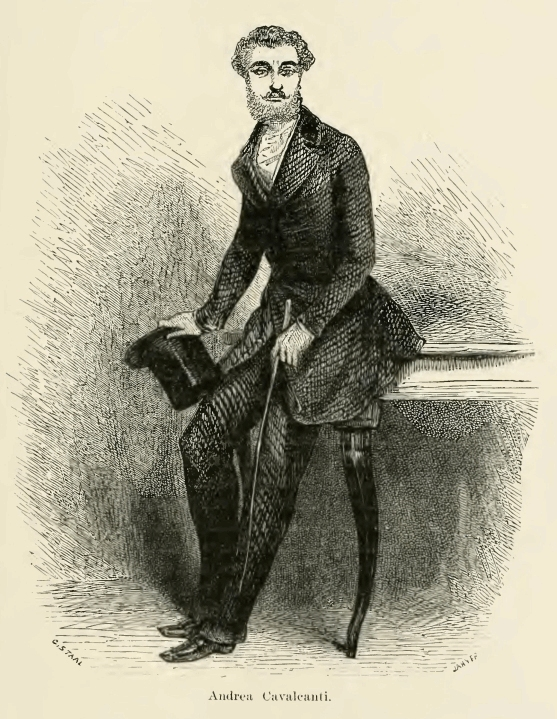
\includegraphics[width=\textwidth]{30133m.jpg}
\end{figure}

“Indeed? Then your father ought to have met with you on the road, for
it is exactly the same route which he himself took, and that is how we
have been able to trace your journey to this place.”

“But,” said Andrea, “if my father had met me, I doubt if he would have
recognized me; I must be somewhat altered since he last saw me.”

“Oh, the voice of nature,” said Monte Cristo.

“True,” interrupted the young man, “I had not looked upon it in that
light.”

“Now,” replied Monte Cristo “there is only one source of uneasiness
left in your father’s mind, which is this—he is anxious to know how you
have been employed during your long absence from him, how you have been
treated by your persecutors, and if they have conducted themselves
towards you with all the deference due to your rank. Finally, he is
anxious to see if you have been fortunate enough to escape the bad
moral influence to which you have been exposed, and which is infinitely
more to be dreaded than any physical suffering; he wishes to discover
if the fine abilities with which nature had endowed you have been
weakened by want of culture; and, in short, whether you consider
yourself capable of resuming and retaining in the world the high
position to which your rank entitles you.”

“Sir!” exclaimed the young man, quite astounded, “I hope no false
report——”

“As for myself, I first heard you spoken of by my friend Wilmore, the
philanthropist. I believe he found you in some unpleasant position, but
do not know of what nature, for I did not ask, not being inquisitive.
Your misfortunes engaged his sympathies, so you see you must have been
interesting. He told me that he was anxious to restore you to the
position which you had lost, and that he would seek your father until
he found him. He did seek, and has found him, apparently, since he is
here now; and, finally, my friend apprised me of your coming, and gave
me a few other instructions relative to your future fortune. I am quite
aware that my friend Wilmore is peculiar, but he is sincere, and as
rich as a gold mine, consequently, he may indulge his eccentricities
without any fear of their ruining him, and I have promised to adhere to
his instructions. Now, sir, pray do not be offended at the question I
am about to put to you, as it comes in the way of my duty as your
patron. I would wish to know if the misfortunes which have happened to
you—misfortunes entirely beyond your control, and which in no degree
diminish my regard for you—I would wish to know if they have not, in
some measure, contributed to render you a stranger to the world in
which your fortune and your name entitle you to make a conspicuous
figure?”

“Sir,” returned the young man, with a reassurance of manner, “make your
mind easy on this score. Those who took me from my father, and who
always intended, sooner or later, to sell me again to my original
proprietor, as they have now done, calculated that, in order to make
the most of their bargain, it would be politic to leave me in
possession of all my personal and hereditary worth, and even to
increase the value, if possible. I have, therefore, received a very
good education, and have been treated by these kidnappers very much as
the slaves were treated in Asia Minor, whose masters made them
grammarians, doctors, and philosophers, in order that they might fetch
a higher price in the Roman market.”

Monte Cristo smiled with satisfaction; it appeared as if he had not
expected so much from M. Andrea Cavalcanti.

“Besides,” continued the young man, “if there did appear some defect in
education, or offence against the established forms of etiquette, I
suppose it would be excused, in consideration of the misfortunes which
accompanied my birth, and followed me through my youth.”

“Well,” said Monte Cristo in an indifferent tone, “you will do as you
please, count, for you are the master of your own actions, and are the
person most concerned in the matter, but if I were you, I would not
divulge a word of these adventures. Your history is quite a romance,
and the world, which delights in romances in yellow covers, strangely
mistrusts those which are bound in living parchment, even though they
be gilded like yourself. This is the kind of difficulty which I wished
to represent to you, my dear count. You would hardly have recited your
touching history before it would go forth to the world, and be deemed
unlikely and unnatural. You would be no longer a lost child found, but
you would be looked upon as an upstart, who had sprung up like a
mushroom in the night. You might excite a little curiosity, but it is
not everyone who likes to be made the centre of observation and the
subject of unpleasant remark.”

“I agree with you, monsieur,” said the young man, turning pale, and, in
spite of himself, trembling beneath the scrutinizing look of his
companion, “such consequences would be extremely unpleasant.”

“Nevertheless, you must not exaggerate the evil,” said Monte Cristo,
“for by endeavoring to avoid one fault you will fall into another. You
must resolve upon one simple and single line of conduct, and for a man
of your intelligence, this plan is as easy as it is necessary; you must
form honorable friendships, and by that means counteract the prejudice
which may attach to the obscurity of your former life.”

Andrea visibly changed countenance.

“I would offer myself as your surety and friendly adviser,” said Monte
Cristo, “did I not possess a moral distrust of my best friends, and a
sort of inclination to lead others to doubt them too; therefore, in
departing from this rule, I should (as the actors say) be playing a
part quite out of my line, and should, therefore, run the risk of being
hissed, which would be an act of folly.”

“However, your excellency,” said Andrea, “in consideration of Lord
Wilmore, by whom I was recommended to you——”

“Yes, certainly,” interrupted Monte Cristo; “but Lord Wilmore did not
omit to inform me, my dear M. Andrea, that the season of your youth was
rather a stormy one. Ah,” said the count, watching Andrea’s
countenance, “I do not demand any confession from you; it is precisely
to avoid that necessity that your father was sent for from Lucca. You
shall soon see him. He is a little stiff and pompous in his manner, and
he is disfigured by his uniform; but when it becomes known that he has
been for eighteen years in the Austrian service, all that will be
pardoned. We are not generally very severe with the Austrians. In
short, you will find your father a very presentable person, I assure
you.”

“Ah, sir, you have given me confidence; it is so long since we were
separated, that I have not the least remembrance of him, and, besides,
you know that in the eyes of the world a large fortune covers all
defects.”

“He is a millionaire—his income is 500,000 francs.”

“Then,” said the young man, with anxiety, “I shall be sure to be placed
in an agreeable position.”

“One of the most agreeable possible, my dear sir; he will allow you an
income of 50,000 livres per annum during the whole time of your stay in
Paris.”

“Then in that case I shall always choose to remain there.”

“You cannot control circumstances, my dear sir; ‘man proposes, and God
disposes.’” Andrea sighed.

“But,” said he, “so long as I do remain in Paris, and nothing forces me
to quit it, do you mean to tell me that I may rely on receiving the sum
you just now mentioned to me?”

“You may.”

“Shall I receive it from my father?” asked Andrea, with some
uneasiness.

“Yes, you will receive it from your father personally, but Lord Wilmore
will be the security for the money. He has, at the request of your
father, opened an account of 5,000 francs a month at M. Danglars’,
which is one of the safest banks in Paris.”

“And does my father mean to remain long in Paris?” asked Andrea.

“Only a few days,” replied Monte Cristo. “His service does not allow
him to absent himself more than two or three weeks together.”

“Ah, my dear father!” exclaimed Andrea, evidently charmed with the idea
of his speedy departure.

“Therefore,” said Monte Cristo feigning to mistake his
meaning—“therefore I will not, for another instant, retard the pleasure
of your meeting. Are you prepared to embrace your worthy father?”

“I hope you do not doubt it.”

\begin{figure}[ht]
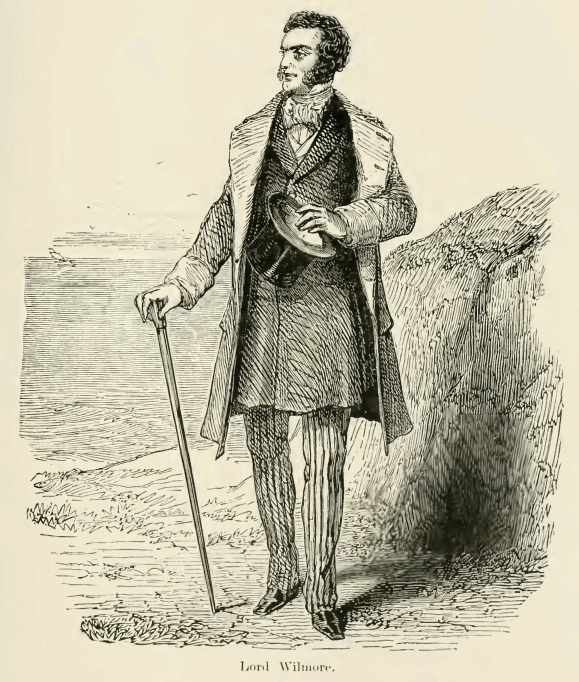
\includegraphics[width=\textwidth]{30137m.jpg}
\end{figure}

“Go, then, into the drawing-room, my young friend, where you will find
your father awaiting you.”

Andrea made a low bow to the count, and entered the adjoining room.
Monte Cristo watched him till he disappeared, and then touched a spring
in a panel made to look like a picture, which, in sliding partly from
the frame, discovered to view a small opening, so cleverly contrived
that it revealed all that was passing in the drawing-room now occupied
by Cavalcanti and Andrea. The young man closed the door behind him, and
advanced towards the major, who had risen when he heard steps
approaching him.

“Ah, my dear father!” said Andrea in a loud voice, in order that the
count might hear him in the next room, “is it really you?”

“How do you do, my dear son?” said the major gravely.

“After so many years of painful separation,” said Andrea, in the same
tone of voice, and glancing towards the door, “what a happiness it is
to meet again!”

“Indeed it is, after so long a separation.”

“Will you not embrace me, sir?” said Andrea.

\begin{figure}[ht]
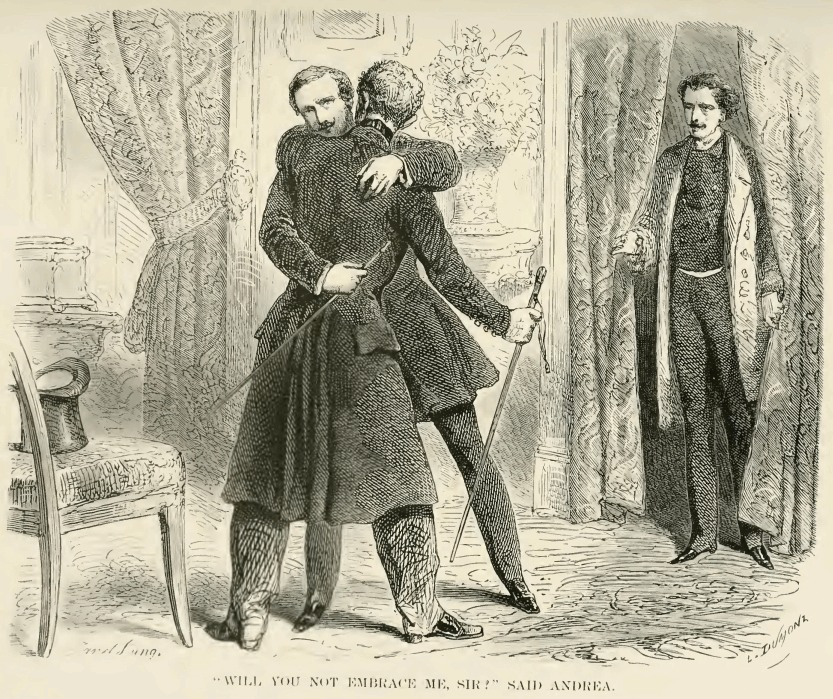
\includegraphics[width=\textwidth]{30139m.jpg}
\end{figure}

“If you wish it, my son,” said the major; and the two men embraced each
other after the fashion of actors on the stage; that is to say, each
rested his head on the other’s shoulder.

“Then we are once more reunited?” said Andrea.

“Once more,” replied the major.

“Never more to be separated?”

“Why, as to that—I think, my dear son, you must be by this time so
accustomed to France as to look upon it almost as a second country.”

“The fact is,” said the young man, “that I should be exceedingly
grieved to leave it.”

“As for me, you must know I cannot possibly live out of Lucca;
therefore I shall return to Italy as soon as I can.”

“But before you leave France, my dear father, I hope you will put me in
possession of the documents which will be necessary to prove my
descent.”

“Certainly; I am come expressly on that account; it has cost me much
trouble to find you, but I had resolved on giving them into your hands,
and if I had to recommence my search, it would occupy all the few
remaining years of my life.”

“Where are these papers, then?”

“Here they are.”

Andrea seized the certificate of his father’s marriage and his own
baptismal register, and after having opened them with all the eagerness
which might be expected under the circumstances, he read them with a
facility which proved that he was accustomed to similar documents, and
with an expression which plainly denoted an unusual interest in the
contents. When he had perused the documents, an indefinable expression
of pleasure lighted up his countenance, and looking at the major with a
most peculiar smile, he said, in very excellent Tuscan:

“Then there is no longer any such thing, in Italy as being condemned to
the galleys?”

The major drew himself up to his full height.

“Why?—what do you mean by that question?”

“I mean that if there were, it would be impossible to draw up with
impunity two such deeds as these. In France, my dear sir, half such a
piece of effrontery as that would cause you to be quickly despatched to
Toulon for five years, for change of air.”

“Will you be good enough to explain your meaning?” said the major,
endeavoring as much as possible to assume an air of the greatest
majesty.

“My dear M. Cavalcanti,” said Andrea, taking the major by the arm in a
confidential manner, “how much are you paid for being my father?”

The major was about to speak, when Andrea continued, in a low voice:

“Nonsense, I am going to set you an example of confidence, they give me
50,000 francs a year to be your son; consequently, you can understand
that it is not at all likely I shall ever deny my parent.”

The major looked anxiously around him.

“Make yourself easy, we are quite alone,” said Andrea; “besides, we are
conversing in Italian.”

“Well, then,” replied the major, “they paid me 50,000 francs down.”

“Monsieur Cavalcanti,” said Andrea, “do you believe in fairy tales?”

“I used not to do so, but I really feel now almost obliged to have
faith in them.”

“You have, then, been induced to alter your opinion; you have had some
proofs of their truth?” The major drew from his pocket a handful of
gold.

“Most palpable proofs,” said he, “as you may perceive.”

“You think, then, that I may rely on the count’s promises?”

“Certainly I do.”

“You are sure he will keep his word with me?”

“To the letter, but at the same time, remember, we must continue to
play our respective parts. I, as a tender father——”

“And I as a dutiful son, as they choose that I shall be descended from
you.”

“Whom do you mean by they?”

“\textit{Ma foi}, I can hardly tell, but I was alluding to those who wrote the
letter; you received one, did you not?”

“Yes.”

“From whom?”

“From a certain Abbé Busoni.”

“Have you any knowledge of him?”

“No, I have never seen him.”

“What did he say in the letter?”

“You will promise not to betray me?”

“Rest assured of that; you well know that our interests are the same.”

“Then read for yourself;” and the major gave a letter into the young
man’s hand. Andrea read in a low voice:

\begin{quote}
{\small“‘You are poor; a miserable old age awaits you. Would you like to
become rich, or at least independent? Set out immediately for Paris,
and demand of the Count of Monte Cristo, Avenue des Champs-Élysées, No.
30, the son whom you had by the Marchesa Corsinari, and who was taken
from you at five years of age. This son is named Andrea Cavalcanti. In
order that you may not doubt the kind intention of the writer of this
letter, you will find enclosed an order for 2,400 francs, payable in
Florence, at Signor Gozzi’s; also a letter of introduction to the Count
of Monte Cristo, on whom I give you a draft of 48,000 francs. Remember
to go to the count on the 26th May at seven o’clock in the evening.

\begin{flushright}
“(Signed) ‘Abbé Busoni.’”
\end{flushright}}
\end{quote}

“It is the same.”

“What do you mean?” said the major.

“I was going to say that I received a letter almost to the same
effect.”

“You?”

“Yes.”

“From the Abbé Busoni?”

“No.”

“From whom, then?”

“From an Englishman, called Lord Wilmore, who takes the name of Sinbad
the Sailor.”

“And of whom you have no more knowledge than I of the Abbé Busoni?”

“You are mistaken; there I am ahead of you.”

“You have seen him, then?”

“Yes, once.”

“Where?”

“Ah, that is just what I cannot tell you; if I did, I should make you
as wise as myself, which it is not my intention to do.”

“And what did the letter contain?”

“Read it.”

\begin{quote}
“‘You are poor, and your future prospects are dark and gloomy. Do you
wish for a name? should you like to be rich, and your own master?’”
\end{quote}

“\textit{Parbleu!}” said the young man; “was it possible there could be two
answers to such a question?”

\begin{quote}
{\small“‘Take the post-chaise which you will find waiting at the Porte de
Gênes, as you enter Nice; pass through Turin, Chambéry, and
Pont-de-Beauvoisin. Go to the Count of Monte Cristo, Avenue des
Champs-Élysées, on the 26th of May, at seven o’clock in the evening,
and demand of him your father. You are the son of the Marchese
Cavalcanti and the Marchesa Oliva Corsinari. The marquis will give you
some papers which will certify this fact, and authorize you to appear
under that name in the Parisian world. As to your rank, an annual
income of 50,000 livres will enable you to support it admirably. I
enclose a draft for 5,000 livres, payable on M. Ferrea, banker at Nice,
and also a letter of introduction to the Count of Monte Cristo, whom I
have directed to supply all your wants.

\begin{flushright}
“‘Sinbad the Sailor.’”
\end{flushright}}
\end{quote}

“Humph,” said the major; “very good. You have seen the count, you say?”

“I have only just left him.”

“And has he conformed to all that the letter specified?”

“He has.”

“Do you understand it?”

“Not in the least.”

“There is a dupe somewhere.”

“At all events, it is neither you nor I.”

“Certainly not.”

“Well, then——”

“Why, it does not much concern us, do you think it does?”

“No; I agree with you there. We must play the game to the end, and
consent to be blindfolded.”

“Ah, you shall see; I promise you I will sustain my part to
admiration.”

“I never once doubted your doing so.” Monte Cristo chose this moment
for re-entering the drawing-room. On hearing the sound of his
footsteps, the two men threw themselves in each other’s arms, and while
they were in the midst of this embrace, the count entered.

“Well, marquis,” said Monte Cristo, “you appear to be in no way
disappointed in the son whom your good fortune has restored to you.”

“Ah, your excellency, I am overwhelmed with delight.”

“And what are your feelings?” said Monte Cristo, turning to the young
man.

“As for me, my heart is overflowing with happiness.”

“Happy father, happy son!” said the count.

“There is only one thing which grieves me,” observed the major, “and
that is the necessity for my leaving Paris so soon.”

“Ah, my dear M. Cavalcanti, I trust you will not leave before I have
had the honor of presenting you to some of my friends.”

“I am at your service, sir,” replied the major.

“Now, sir,” said Monte Cristo, addressing Andrea, “make your
confession.”

“To whom?”

“Tell M. Cavalcanti something of the state of your finances.”

“\textit{Ma foi!} monsieur, you have touched upon a tender chord.”

“Do you hear what he says, major?”

“Certainly I do.”

“But do you understand?”

“I do.”

“Your son says he requires money.”

“Well, what would you have me do?” said the major.

“You should furnish him with some of course,” replied Monte Cristo.

“I?”

“Yes, you,” said the count, at the same time advancing towards Andrea,
and slipping a packet of bank-notes into the young man’s hand.

“What is this?”

“It is from your father.”

“From my father?”

“Yes; did you not tell him just now that you wanted money? Well, then,
he deputes me to give you this.”

“Am I to consider this as part of my income on account?”

“No, it is for the first expenses of your settling in Paris.”

“Ah, how good my dear father is!”

“Silence,” said Monte Cristo; “he does not wish you to know that it
comes from him.”

“I fully appreciate his delicacy,” said Andrea, cramming the notes
hastily into his pocket.

“And now, gentlemen, I wish you good-morning,” said Monte Cristo.

“And when shall we have the honor of seeing you again, your
excellency?” asked Cavalcanti.

“Ah,” said Andrea, “when may we hope for that pleasure?”

“On Saturday, if you will—Yes.—Let me see—Saturday—I am to dine at my
country house, at Auteuil, on that day, Rue de la Fontaine, No. 28.
Several persons are invited, and among others, M. Danglars, your
banker. I will introduce you to him, for it will be necessary he should
know you, as he is to pay your money.”

“Full dress?” said the major, half aloud.

“Oh, yes, certainly,” said the count; “uniform, cross, knee-breeches.”

“And how shall I be dressed?” demanded Andrea.

\begin{figure}[ht]
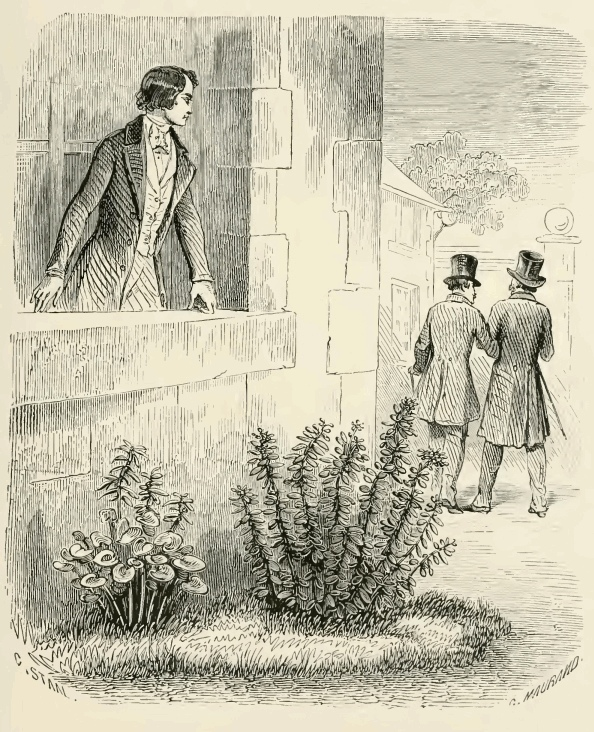
\includegraphics[width=\textwidth]{30145m.jpg}
\end{figure}

“Oh, very simply; black trousers, patent leather boots, white
waistcoat, either a black or blue coat, and a long cravat. Go to Blin
or Véronique for your clothes. Baptistin will tell you where, if you do
not know their address. The less pretension there is in your attire,
the better will be the effect, as you are a rich man. If you mean to
buy any horses, get them of Devedeux, and if you purchase a phaeton, go
to Baptiste for it.”

“At what hour shall we come?” asked the young man.

“About half-past six.”

“We will be with you at that time,” said the major. The two Cavalcanti
bowed to the count, and left the house. Monte Cristo went to the
window, and saw them crossing the street, arm in arm.

“There go two miscreants;” said he, “it is a pity they are not really
related!” Then, after an instant of gloomy reflection, “Come, I will go
to see the Morrels,” said he; “I think that disgust is even more
sickening than hatred.”

\begin{figure}[ht]
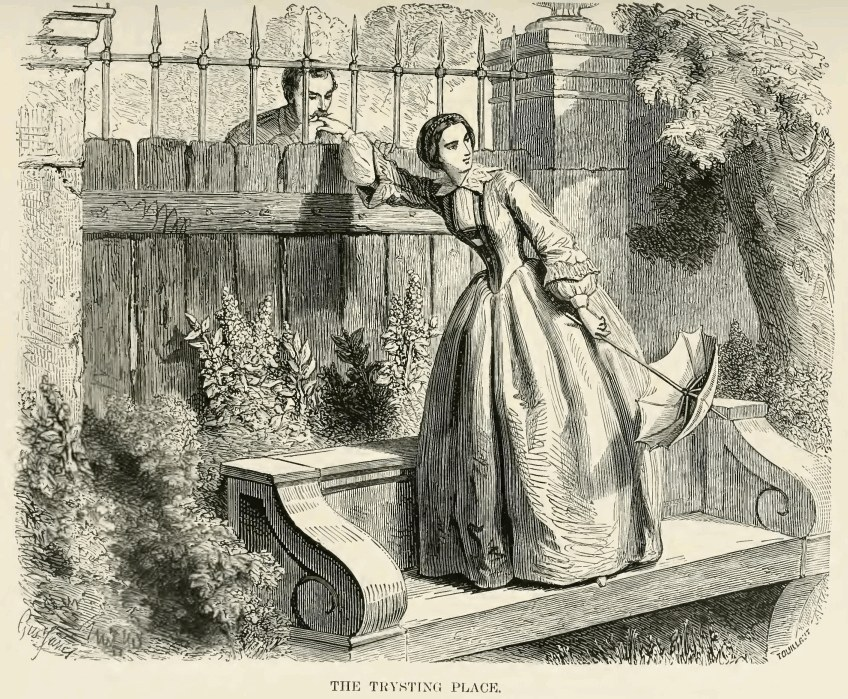
\includegraphics[width=\textwidth]{30147m.jpg}
\end{figure}
